In this chapter, we explore the construction and implementation of a simulation designed to evaluate the proposed improvement strategy for the CRC care pathway within the Southern Metropolitan Public Healthcare System. This simulation serves as a crucial tool in assessing the feasibility, costs, and potential outcomes of the proposed enhancements outlined in the preceding chapters.

The simulation model was written entirely on Python. All of its code is available on this public github repository.

\url{https://github.com/Tomasalvarez15/crc_screening_simulator}

\section{Simulation Framework Selection}

The selection of framework for the simulation model started with a revision of the available type of models for this kind of simulation. A recent study found 43 other studies which used a simulation model to validate a screening strategy for CRC \cite{smith_simulation_2020}. Of them the most used kind of model was Markov modeling (72\%), Monte Carlo modeling (16\%) and microsimulation (14\%). It is important to note that some studies used more than one kind of model. 33\% of the studies cited the MISCAN-Colon model \cite{loeve_miscan-colon_1999} as their base model.

The other simulation models considered did not align with the specific requirements of this study. The Markov model, for instance, lacks the capability to incorporate dynamic disease progression and is not easily scalable over the long term. Given the objective of accurately representing the natural history of colorectal cancer, this model was deemed unsuitable. Similarly, Monte Carlo simulations sequentially run each individual's life, making them less conducive to simulating all individuals simultaneously, as desired for this investigation. While Discrete Event Simulation (DES) was a viable option, its focus on how individual actions impact the system differs from the individual-centric approach of microsimulation. Consequently, microsimulation emerged as the preferred simulation type for this study due to its emphasis on capturing the nuanced dynamics of individual experiences within the broader healthcare system.

\section{Microsimulation Model Operational Explanation}

The microsimulation model functions as a virtual population filled with individuals. It begins at a specified starting year and progresses until a set number of years have elapsed, collecting statistics for later analysis. The simulation depicts the lives of individuals in the population, modeling the screening process for those who undergo it and simulating the natural history of CRC for those who develop the disease. Individuals who do not fall into these categories remain in the simulation without active interaction until their simulated death.

Next, each component of the simulation's structure and processes will be explained in detail.

\subsection*{Structure of the Simulation Objects}

The microsimulation has two main structures. The population and the individuals. Each of them have specific properties and functions that allow the simulation to represent the behaviour of CRC care.

\begin{figure}[H]
    \centering
    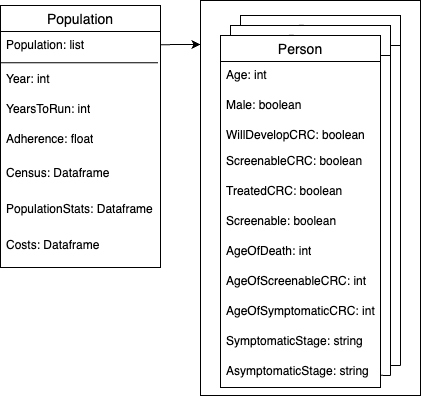
\includegraphics[scale=0.6]{images/4.simulation/ClassDiagram.png}
    \caption{Structure of the Simulation Objects and their Attributes with Types}
    \label{fig:structure_of_the_simulation_objects}
\end{figure}

The diagram in Figure \ref{fig:structure_of_the_simulation_objects} shows the essential data retained by the Population object. Firstly, it includes a list of all individuals. Secondly, it contains the current year and adherence percentage for generating new individuals. Thirdly, it tracks the remaining years to determine the simulation's end. Fourthly, it maintains the Census, PopulationStats, and Costs DataFrames for recording yearly statistics like age distributions, activity records, and operational costs.

Each Person object encapsulates all required information to depict an individual's current state, encompassing factors such as age, sex, anticipated age of death, and pertinent variables concerning CRC diagnosis and progression.

\subsection*{Instantiating a Person Object}
 

When creating a Person object, certain attributes are pre-set, while others are determined by random uniform distributions. If these attributes fall below specific parameters, they are assigned one value; otherwise, they are assigned another.

\begin{figure}[H]
    \centering
    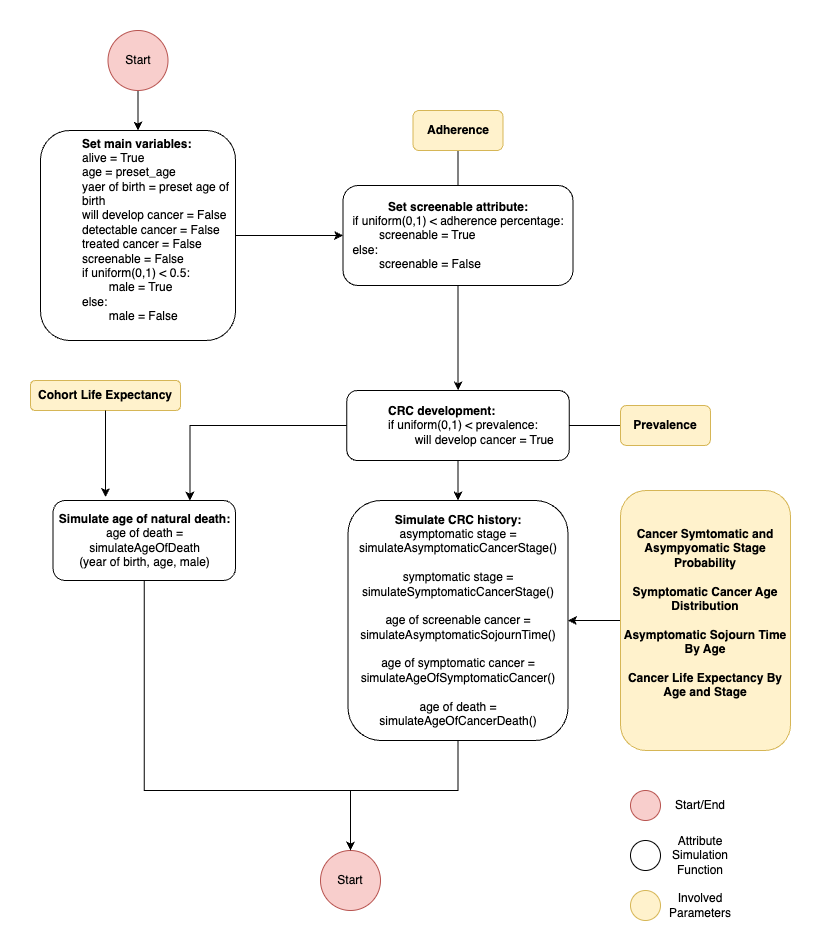
\includegraphics[scale=0.4]{images/4.simulation/InstantiatingAPerson.png}
    \caption{Instantiating a Person Object Process}
    \label{fig:instantiating_a_person}
\end{figure}

As shown in Figure \ref{fig:instantiating_a_person}, several parameters are considered when simulating each individual's life. Once created, their attributes are set, including the ages at which they will experience changes in status.

\begin{figure}[H]
    \centering
    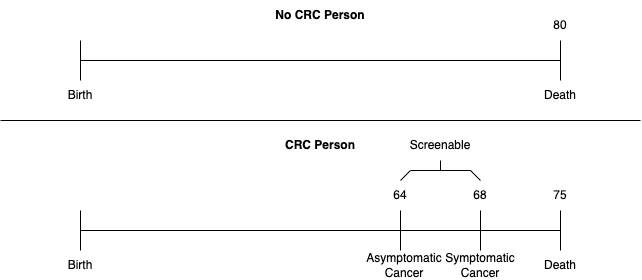
\includegraphics[width=1\textwidth]{images/4.simulation/NaturalHistoryDiagram.png}
    \caption{Person Life History from the Simulation}
    \label{fig:natural_history}
\end{figure}

In Figure \ref{fig:natural_history}, individuals without CRC experience no status changes except for their eventual death at a specified age. However, for those with CRC, a positive screening result within the screenable interval recalculates their life expectancy. Detecting CRC earlier extends their life, recorded as years gained from screening. If their life expectancy decreases due to a later asymptomatic stage, the years are subtracted from the total.

\subsection*{Yearly Progression Overview}
The program progresses through each year (iteration), checking and updating the health status of each person in the population. This process repeats for each simulated year, allowing researchers to observe how different screening strategies impact the overall CRC outcomes in the population over time.

The decision to run the microsimulation in one-year intervals balances capturing meaningful changes in CRC progression with maintaining computational efficiency. While shorter intervals would increase complexity and computational load, this enhancement could be added to the simulation model in the future.

\begin{figure}[H]
    \centering
    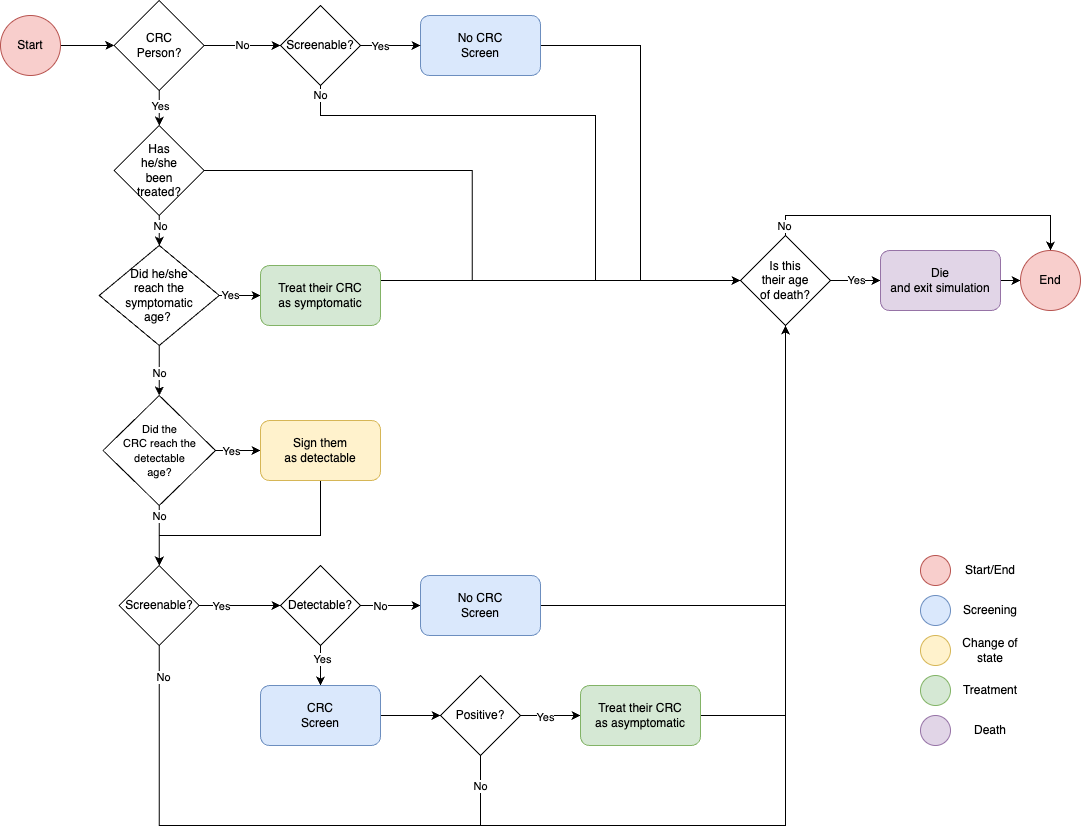
\includegraphics[width=1\textwidth]{images/4.simulation/simulation_person_process.png}
    \caption{Person Processing Flowchart}
    \label{fig:simulation_person_processing}
\end{figure}

Each year, every individual undergoes the process depicted in Figure \ref{fig:simulation_person_processing}. In the first step, this pathway segregates those with CRC in their natural history.

For individuals without CRC, their significance lies primarily in the statistics of screening strategies, as the majority of screenings are conducted on individuals who will never develop CRC.

For those with CRC in their natural history, their course of action depends on the stage of their disease and whether they are screenable. They may undergo screening and/or treatment either symptomatically, when the disease manifests symptoms, or asymptomatically, when CRC is detected through the screening process. If this happens, their age of death will be updated according to their asymptomatic stage.

\section{Simulation Parameters}
\label{section:simulation_parameters}

For the simulation to be accurate, multiple data is needed in various aspects. Initially, we will examine demographic data, followed by data related to the CRC disease, and finally, the costs of procedures for the economic analysis.

\subsection{Demographic Data}

For demographic data, the initial population was obtained from the studied region, and the population projection from Chile was available. However, the best publicly available information for cohort life expectancy came from the US. Replacing this data with sources from Chile, ideally from the studied region, is an important endeavor for improving the accuracy of the simulation.


\subsubsection*{Initial Population}

To simulate the current population the MND team provided a dataset which contained the number of individuals by age from the district that were registered in the public healthcare system in the year 2023. The district contains a total of 1122870 people registered to the public healthcare system. Figure \ref{fig:registered_vs_age} presents a plot depicting the distribution of registered individuals by age in 2023.

\begin{figure}[H]
    \centering
    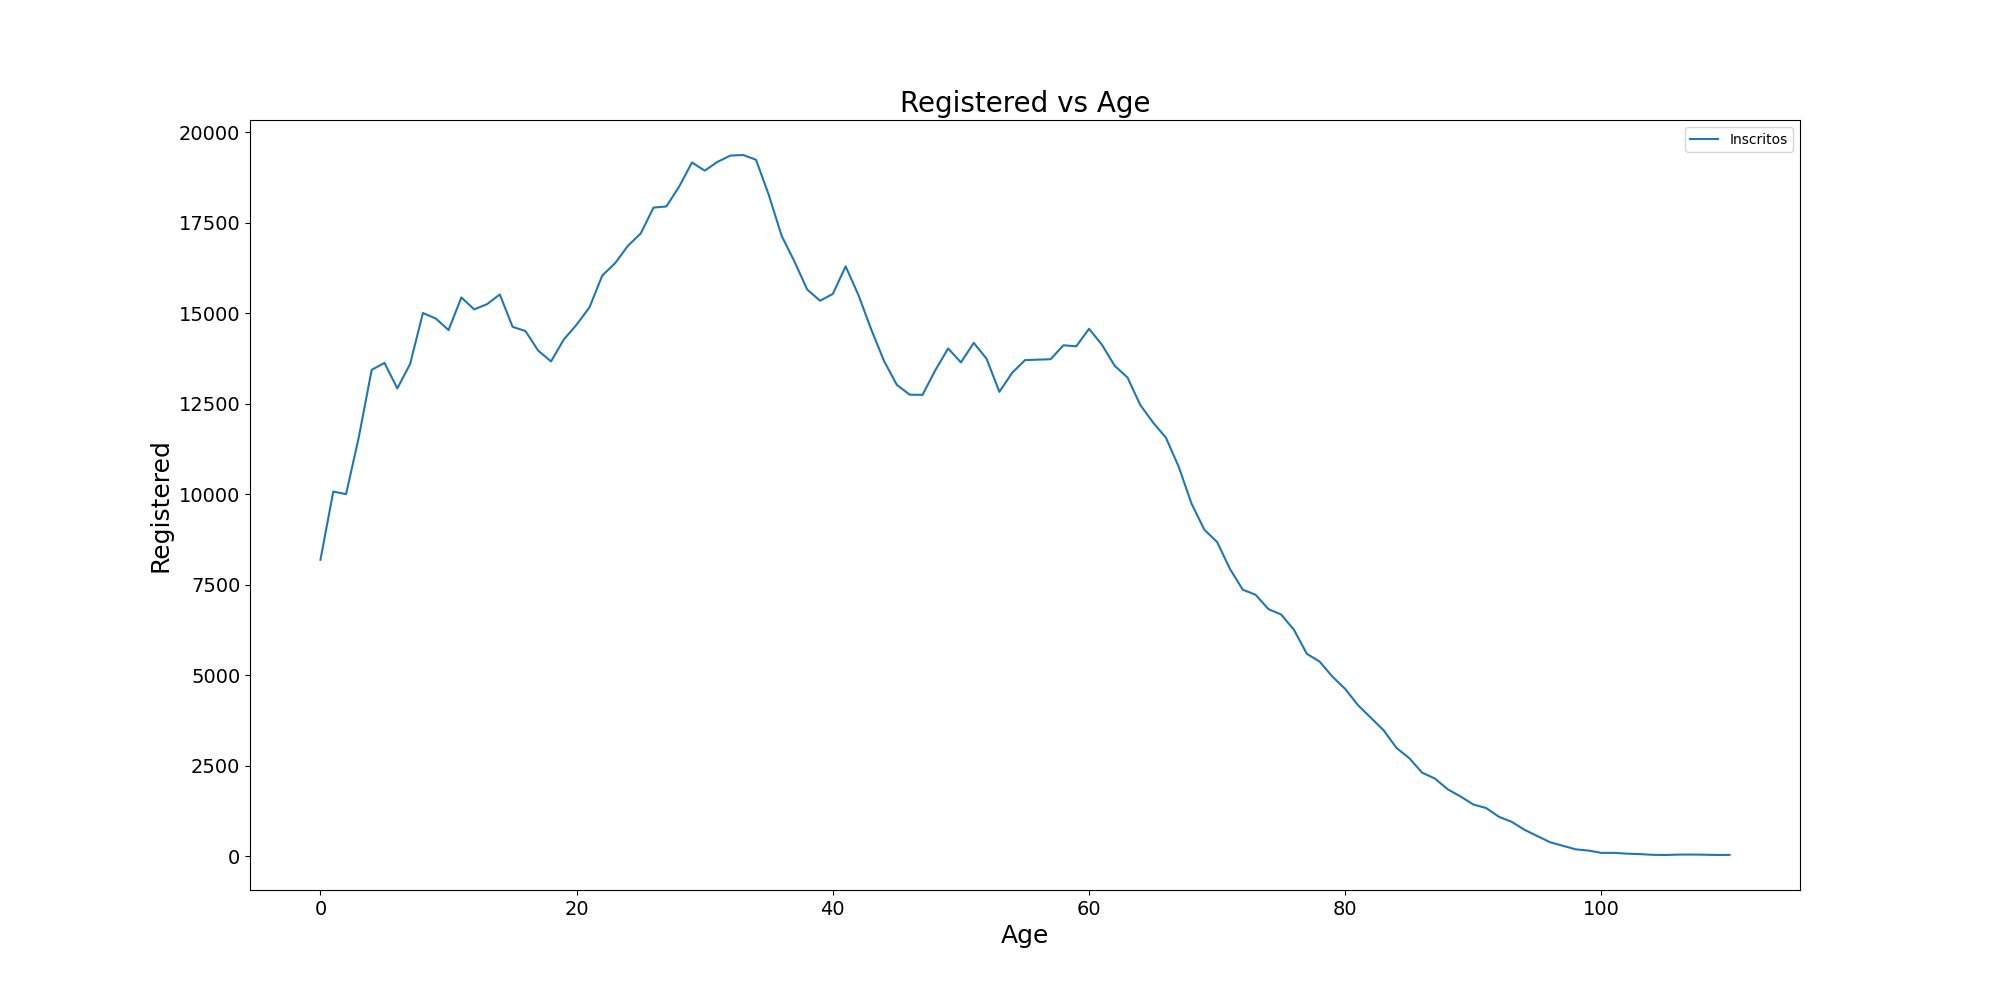
\includegraphics[width=1\textwidth]{images/4.simulation/Registered_vs_Age.png}
    \caption{Registered vs Age from SMPHS in 2023}
    \label{fig:registered_vs_age}
\end{figure}

\subsubsection*{Public Healthcare Registrations}

To sustain the population over time, new individuals must register in the public healthcare system each year. Figure \ref{fig:registered_vs_age} illustrates that many individuals are not registered at birth.

\begin{figure}[H]
    \centering
    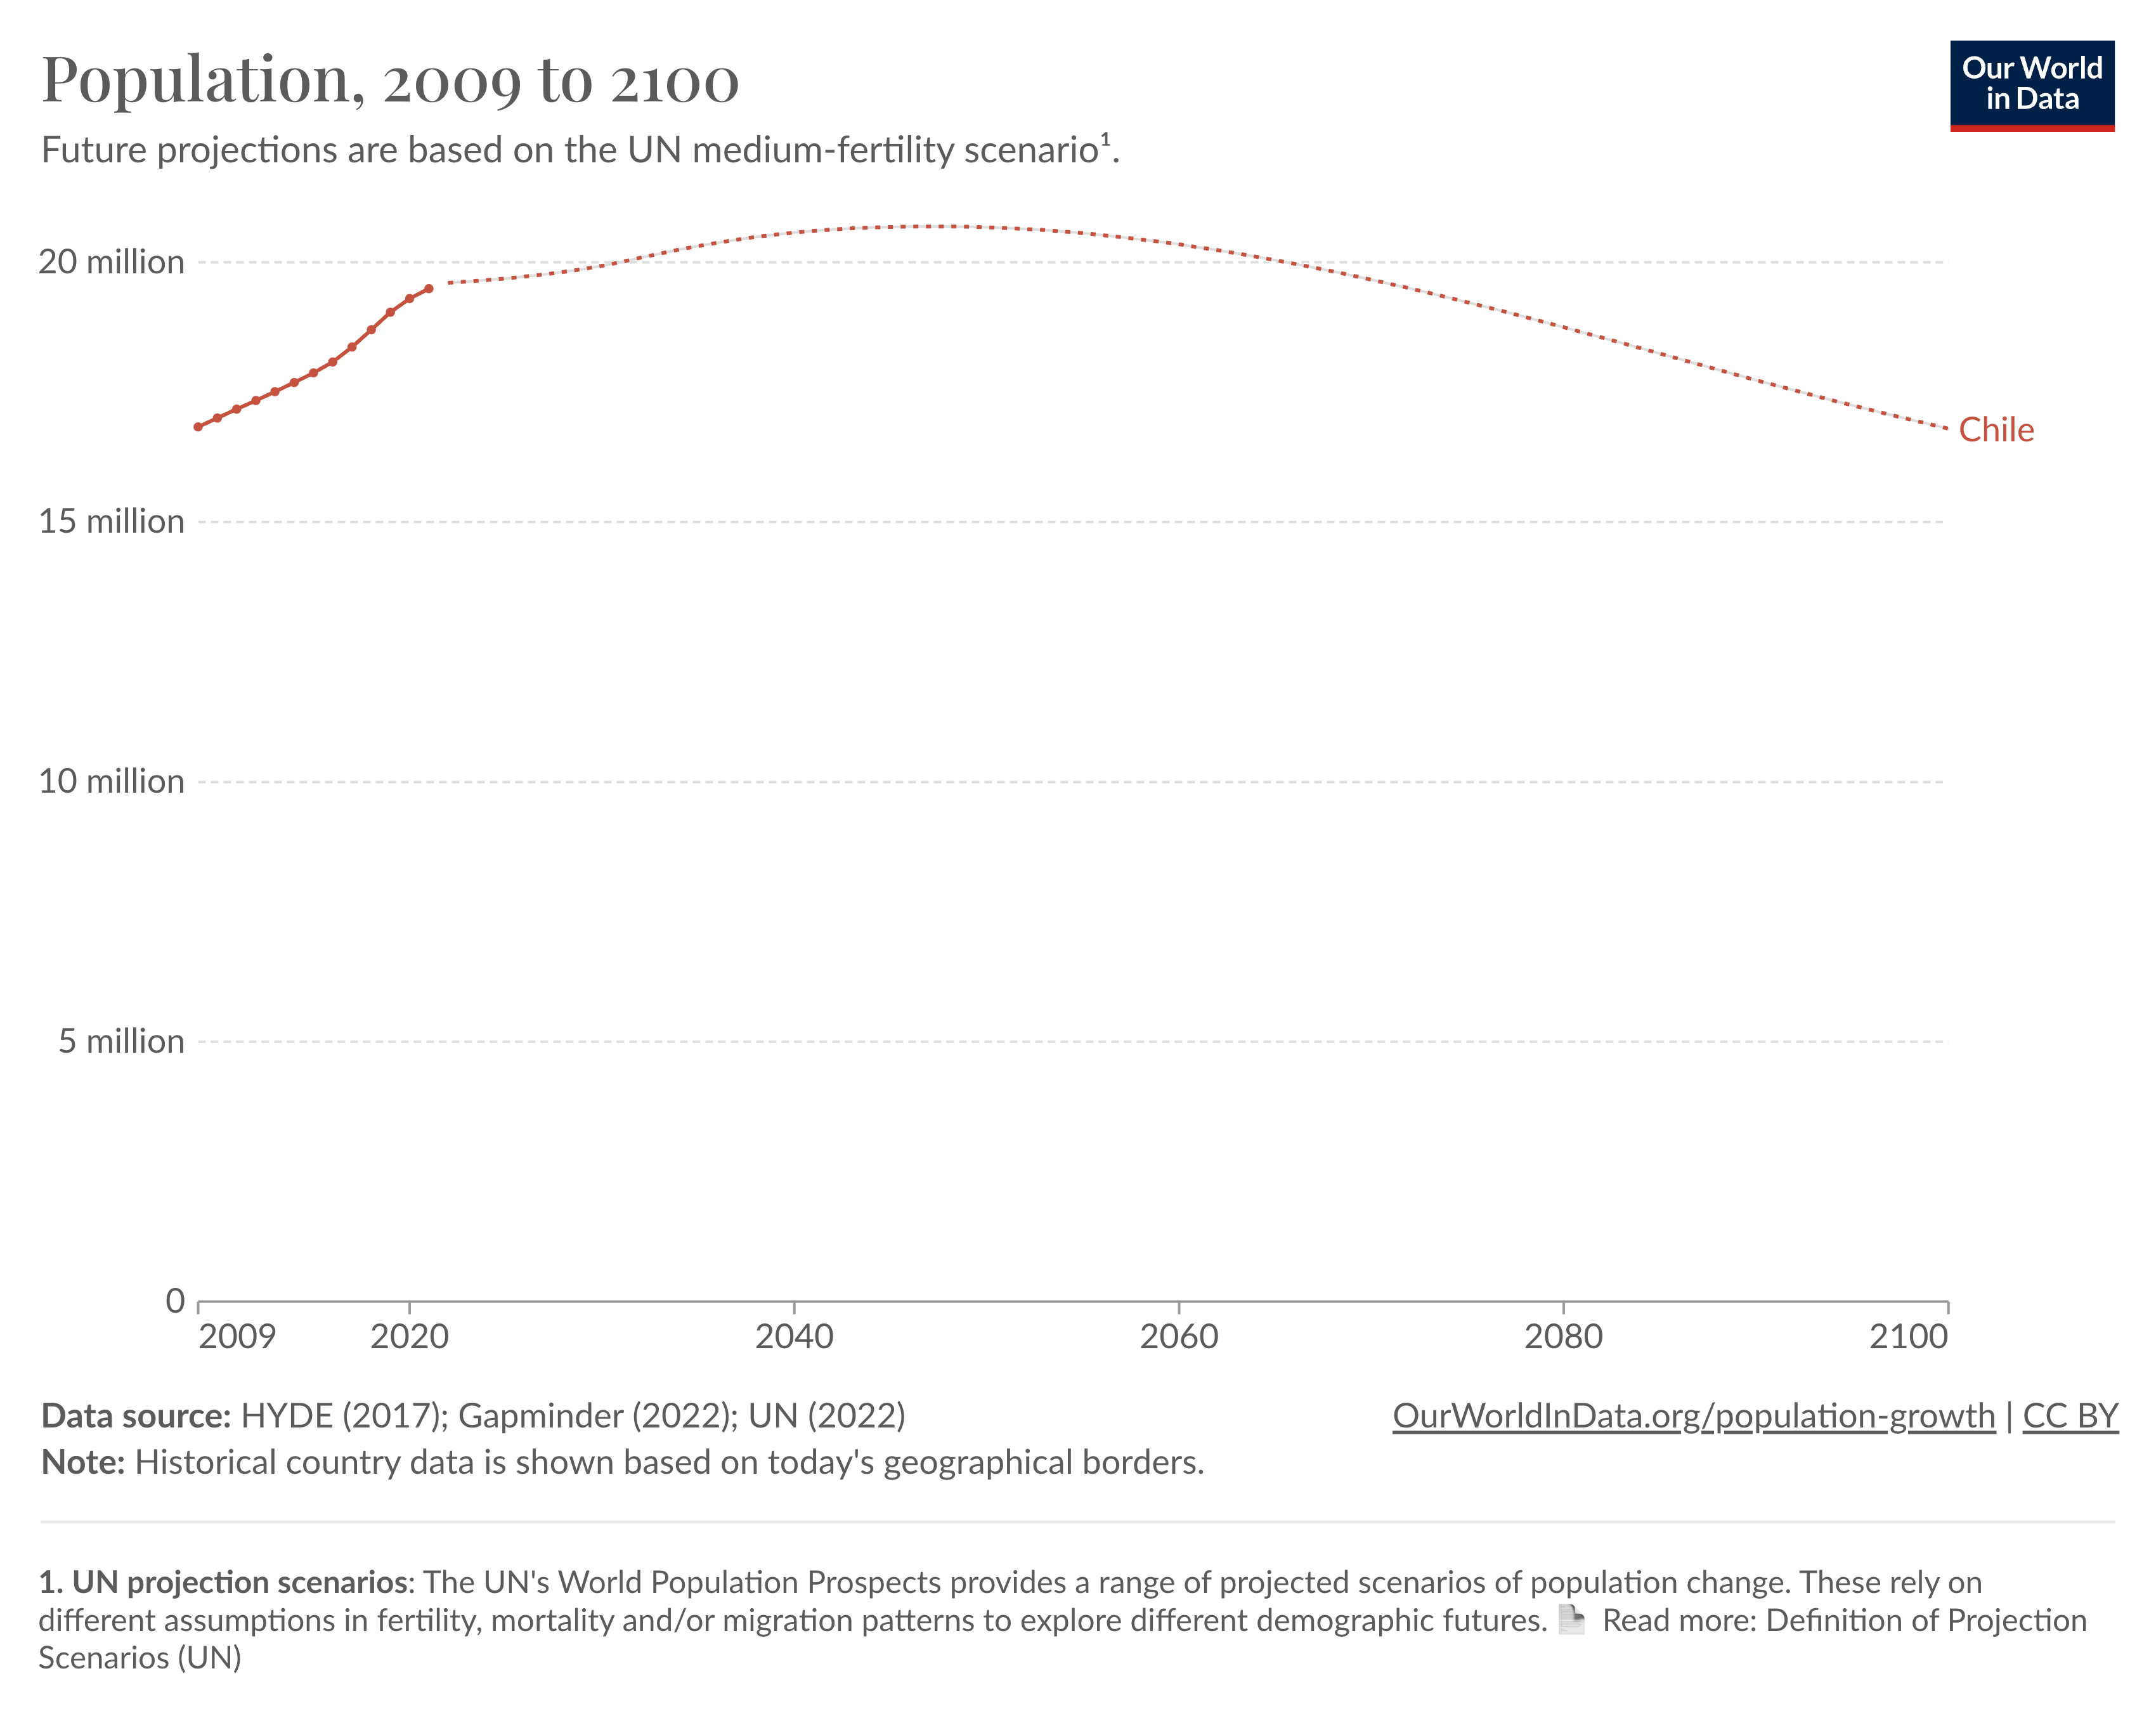
\includegraphics[width=1\textwidth]{images/4.simulation/chile_population_projection.png}
    \caption{Chilean Population Projection\textsuperscript{1}}
    \label{fig:chilean_population_projection}
\end{figure}

\footnotetext[1]{From \textit{Population Projection}. Our World on Data, 2023. \url{https://ourworldindata.org/grapher/population-long-run-with-projections?time=2009..latest&country=~CHL}}

As shown in Figure \ref{fig:chilean_population_projection}, the Chilean population is expected to grow over the next 20 years before gradually declining. Given that the growth and decline trends are neither significant nor reliable, this population trend was considered insignificant for the simulation. Therefore, the goal is to maintain a constant registered population.

\begin{table}[H]
\caption{Registrations per year in the Simulation}
\centering
\begin{tabular}{|c|c|}
\hline
Age Interval & Number of Births\\ \hline
0 & Normal(9000, 500)\\ \hline
1-8 & Normal(3200, 300)\\ \hline
21-30 & Normal(1800, 300)\\ \hline
\end{tabular}

\label{table:registrations_per_year}
\end{table}

The approach works by establishing constant birth rates, with slight random deviations, across different age intervals. This approach ensures the distribution of registered individuals remains consistent, as demonstrated in Table \ref{table:registrations_per_year}.

\subsubsection*{Cohort Life Expectancy}

To ensure accurate simulation of individual lifespans, access to cohort life expectancy data is crucial. While traditional life expectancy figures provide an average lifespan for a population, our simulation required more specific cohort-based data, detailing the average lifespan of individuals born in particular years. 

Although such data for the Chilean population was available publicly, it had limitations, covering the years 1992 to 2050 and extending to one hundred years of age \cite{noauthor_proyecciones_2024}. In contrast, the US national Social Security database offered a more comprehensive dataset, spanning from 1900 to 2095 and including both real and simulated life expectancies up to age 119. Due to its broader range and depth, the US dataset was considered more suitable for our simulation. Despite attempts to obtain extended data from the Chilean National Statistics Institute, no response was received.

Due to the extensive nature of the dataset, comprising 23,520 rows and 14 columns, detailed tables are not included in this thesis but can be accessed through the US Social Security Administration Site \cite{noauthor_social_2024}.

\begin{figure}[H]
    \centering
    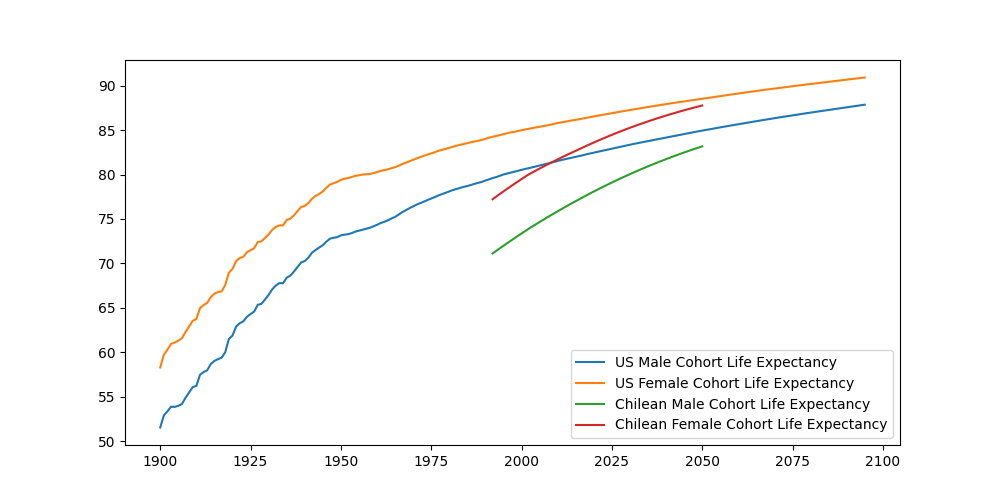
\includegraphics[width=1\textwidth]{images/4.simulation/cohort_life_expectancy.png}
    \caption{Cohort Life Expectancy}
    \label{fig:cohort_life_expectancy}
\end{figure}

Figure \ref{fig:cohort_life_expectancy} confirms the wider age range covered by the US data compared to the Chilean dataset. However, it also reveals a notable difference in life expectancy between the two populations. Although this gap may not greatly influence the simulation's results, it does raise concerns about the datasets' compatibility. This difference underscores the need to carefully review and possibly adjust other data points in the simulation to ensure they align with the unique characteristics of the Chilean population.

\subsection{CRC Disease Parameters}

All the data sources for CRC in this study are from outside Chile. This raises concerns, as the behavior of CRC can vary significantly by region. Factors like age, sex, smoking, and body mass index influence CRC incidence rates and differ across regions, as highlighted by \citeA{doubeni_contribution_2012}. Additionally, race and geographic location also impact CRC incidence, as shown by \citeA{wang_geographic_2023}. Ideally, comparable data will become available in Chile to ensure more accurate regional representation in the future.

\subsubsection*{Prevalence}

Determining whether an individual will develop colorectal cancer during their lifetime is a critical aspect of the simulation process. However, obtaining accurate data for this probability, particularly for the Chilean population, poses a challenge. While prevalence and incidence rates are commonly available, specific lifetime risk data is scarce. In Chile, the projected incidence rate stands at 20.4 cases per 100,000 inhabitants, according to the most recent data \cite{rios_situacion_2020}. Nonetheless, the most reliable indicator of lifetime risk was sourced from the United States, where it's reported as 4.4\% for men and 4.1\% for women \cite{siegel_cancer_2020}. These lifetime risk parameters are detailed in Table \ref{table:crc_lifetime_risk}.

\begin{table}[H]
\caption{Lifetime Risk of developing CRC}
\centering
\begin{tabular}{|c|c|}
\hline
Sex & Lifetime Risk\\ \hline
Male & 4.4\%\\ \hline
Female & 4.1\%\\ \hline
Average & 4.25\%\\ \hline
\end{tabular}
\label{table:crc_lifetime_risk}
\end{table}

\subsubsection*{Cancer Stage on Symptomatic or Asymptomatic Detection}

The simulation determines, when generating each individual, at which stage their cancer will be detected, either asymptomatically or symptomatically. This probability for each stage was derived from a study in the Netherlands. This study compared the stage distribution of CRC patients whose disease was detected by symptoms versus those detected by a fecal occult blood test (FOBT) screening strategy \cite{van_rossum_earlier_2009}.

\begin{figure}[H]
    \centering
    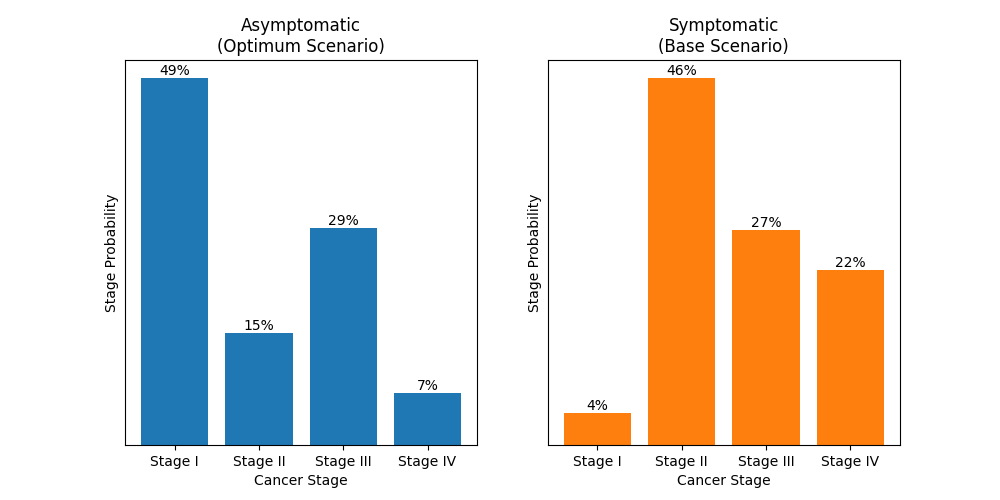
\includegraphics[width=1\textwidth]{images/4.simulation/cancer_stage_probability.png}
    \caption{Symptomatic or Asymptomatic Detection}
    \label{fig:symptomatic_vs_asymptomatic_detection}
\end{figure}

The distribution of asymptomatic and symptomatic cancer stages is illustrated in Figure \ref{fig:symptomatic_vs_asymptomatic_detection}. In the asymptomatic graph, the optimum scenario is depicted, where all detections occur without symptoms. Conversely, the base case scenario represents a situation where all detections occur due to symptoms, similar to the current state in the SMPHS.

The effectiveness of the screening strategy is reflected in the percentage of asymptomatic detections. As this percentage increases, the distribution of cancer stages will shift closer to the optimum scenario and further from the base case.

\subsubsection*{Symptomatic Age Expectancy}

The first event simulated in CRC individuals is the age at which they develop symptoms of the disease. This step requires data on CRC cases by age.

Unfortunately, the available data on CRC cases by age in Chile was insufficient and lacked the necessary detail for our simulation model. To address this limitation, we sourced the age distribution of new cases from the US Cancer Statistics site \cite{noauthor_uscs_2024}. This dataset provides a comprehensive breakdown by age group, allowing for a more detailed representation of CRC incidence. The extracted age distribution is presented in Table \ref{table:cases_by_age_group}.
\begin{table}[H]
\caption{USA CRC Cases by Age Group}
\centering
\begin{tabular}{|c|c|c|c|}
\hline
Age Group & Cases & Age Group & Cases\\ \hline
1-4       & 0     & 45-49     & 6861\\ \hline
5-9       & 18    & 50-54     & 11429\\ \hline
10-14     & 130   & 55-59     & 12564\\ \hline
15-19     & 259   & 60-64     & 15475\\ \hline
20-24     & 421   & 65-69     & 16809\\ \hline
25-29     & 731   & 70-74     & 16069\\ \hline
30-34     & 1452  & 75-79     & 13502\\ \hline
35-39     & 2471  & 80-84     & 11168\\ \hline
40-44     & 3949  & 85-120    & 12933\\ \hline
\end{tabular}
\label{table:cases_by_age_group}
\end{table}

\subsubsection*{Asymptomatic Screenable Sojourn Time}

It's crucial to simulate the period when CRC is detectable but not yet symptomatic. To address this, a study using the German National Screening Colonoscopy Database was reviewed, providing insights into the sojourn time of the preclinical stage of CRC \cite{brenner_sojourn_2011}. The study detailed age groups and sojourn times by sex, as outlined in Table \ref{table:asymptomatic_sojourn_time}.

\begin{table}[H]
\caption{CRC Asymptomatic Screenable Sojourn Time}
\centering
\begin{tabular}{|c|c|c|}
\hline
Age Group & Male Sojourn Time (95\% CI) & Female Sojourn Time (95\% CI) \\ \hline
0-59   & 5.5 (5.1, 6.0) & 4.7 (4.3, 5.1)\\ \hline
60-64  & 5.2 (4.9, 5.5) & 4.5 (4.1, 4.8)\\ \hline
65-69  & 4.7 (4.5, 4.9) & 4.6 (4.3, 4.8)\\ \hline
70-74  & 4.9 (4.6, 5.1) & 4.8 (4.5, 5.1)\\ \hline
75-79  & 5.0 (4.7, 5.3) & 5.2 (4.8, 5.6)\\ \hline
80-120 & 5.5 (5.0, 6.0) & 5.8 (5.3, 6.3)\\ \hline
\end{tabular}
\label{table:asymptomatic_sojourn_time}
\end{table}

\subsubsection*{CRC Life Expectancy}

It's necessary to simulate the years from the symptomatic detection until the passing of the individual. We used data from a study from the Netherlands which has the life expectancy of CRC patients depending on the stage and the age it was detected \cite{soerjomataram_most_2012}. 

\begin{table}[H]
\caption{CRC Life Expectancy by Sex and Stage}
\centering
\begin{tabular}{|c|c|c|}
\hline
Stage \& Age & Male & Female\\ \hline
I   & 25.3 & 29.8 \\ \hline
II  & 19.2 & 20.9 \\ \hline
III & 13.6 & 16.8 \\ \hline
IV  & 2.1  & 2.2  \\ \hline
\end{tabular}
\label{table:crc_life_expectancy_by_stage}
\end{table}

\begin{table}[H]
\caption{CRC Life Expectancy by Sex and Age}
\centering
\begin{tabular}{|c|c|c|}
\hline
Age & Male & Female\\ \hline
50  & 12.3 & 13.3 \\ \hline
65  & 9.4  & 11.5 \\ \hline
80  & 5.5  & 7    \\ \hline
\end{tabular}
\label{table:crc_life_expectancy_by_age}
\end{table}

The data provided in Tables \ref{table:crc_life_expectancy_by_stage} and \ref{table:crc_life_expectancy_by_age} were utilized to formulate a function capable of determining life expectancy based on both the stage of CRC and the individual's age. This function was developed through interpolation, calculating life expectancy for ages ranging from 1 to 120 years. To achieve this, the stage and age parameters were averaged using dynamically assigned weights. At birth (0 years old), the stage weight is set at 20\%, incrementing linearly until reaching 100\% at 120 years old. The resulting life expectancies generated by this function are graphically depicted in Figures \ref{fig:crc_male_life_expectancies} and \ref{fig:crc_female_life_expectancies}.

\begin{figure}[H]
    \centering
    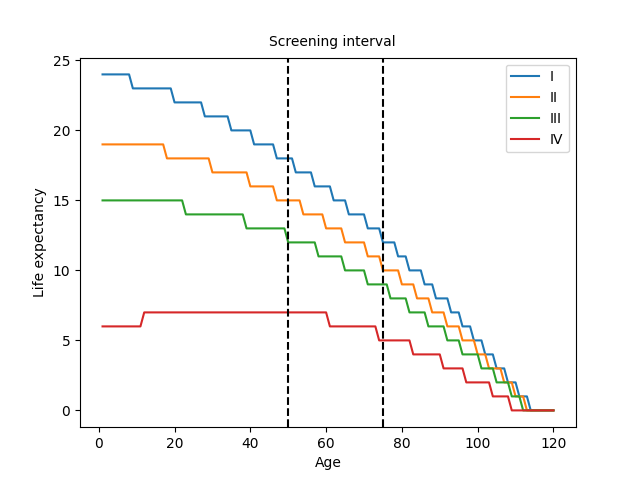
\includegraphics[width=1\textwidth]{images/4.simulation/crc_male_life_expectancies.png}
    \caption{Male CRC Life Expectancies by Age and Stage}
    \label{fig:crc_male_life_expectancies}
\end{figure}

\begin{figure}[H]
    \centering
    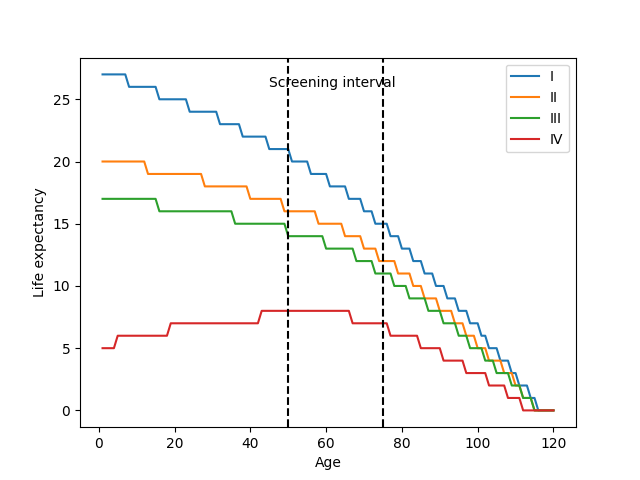
\includegraphics[width=1\textwidth]{images/4.simulation/crc_female_life_expectancies.png}
    \caption{Female CRC Life Expectancies by Age and Stage}
    \label{fig:crc_female_life_expectancies}
\end{figure}

When colorectal cancer is detected while still asymptomatic, the patient's expected age of death is recalculated based on the asymptomatic stage. This adjustment accounts for any difference in years between the original prognosis and the recalculated age, contributing to the overall "years gained" statistic. 

Although this recalibration occasionally results in progression to a more advanced stage, such instances are rare. Moreover, across a wide range of cases analyzed, the cumulative years gained through this strategy consistently show positive outcomes in the long term.

\subsubsection*{Screening Exam}

It was decided that the screening test had to be a fecal immunochemical test (FIT) as it shows better performance compared to the fecal occult blood test (FOBT) \cite{zhu_comparison_2010} in every exam indicator.

This test is being offered by the private sector UC Christus clinic network which has the FIT exam in three variants, with one, two and three samples. As the two and three-sample tests have twice and thrice the value of the single sample test, and the performance indicators don’t seem to improve with more than one sample \cite{amitay_fecal_2019}, the one sample test is the exam chosen for this strategy.

For the tests sensitivity and specificity we used a study that did a Systematic Review and Meta-analysis of many FIT studies \cite{lee_accuracy_2014} which found the values of performance characteristics presented in Table \ref{table:fit_performance_characteristics}.

\begin{table}[H]
\caption{FIT Performance Characteristics}
\centering
\begin{tabular}{|c|c|}
\hline
Performance Characteristic & Value (95\% CI)\\ \hline
Sensitivity & 0.79 (0.69, 0.86)\\ \hline
Specificity & 0.94 (0.92, 0.95)\\ \hline
\end{tabular}
\label{table:fit_performance_characteristics}
\end{table}

\subsubsection*{Adherence to Screening Strategy}

Adherence to screening strategies significantly impacts their effectiveness. Various countries, primarily in Europe, have implemented similar screening approaches, each with different levels of adherence and outcomes \cite{navarro_colorectal_2017}.

\begin{table}[H]
\caption{Countries Screening Strategy Adherences}
\centering
\begin{tabular}{|c|c|c|c|}
\hline
Country     & Adherence & Country & Adherence\\ \hline
Canada         & 16.1\% & California (USA)& 48.2\% \\ \hline
Croatia        & 19.9\% & Ireland         & 51\%   \\ \hline
South Korea    & 21\%   & England         & 52\%   \\ \hline
Taiwan         & 21.4\% & Italy           & 54.4\% \\ \hline
Czech Republic & 22.7\% & Slovenia        & 60.43\%\\ \hline
France         & 36.1\% & Thailand        & 62.9\% \\ \hline
Australia      & 45.4\% & Netherlands     & 68.2\% \\ \hline
Lithuania      & 46\%   &  &  \\ \hline
\end{tabular}
\label{table:countries_adherence_percentage}
\end{table}

As depicted in Table \ref{table:countries_adherence_percentage}, adherence rates for CRC screening vary significantly across different countries, typically falling within the range of 20\% to 60\%. For the simulation in this study, eight adherence scenarios were selected. Taking a cautious approach, an initial adherence rate of 20\% was chosen, reflecting the limited experience of the Chilean government and healthcare system in implementing preventive medicine programs. The first five scenarios represent the incremental introduction of the screening strategy at adherence rates of 0\%, 5\%, 10\%, 15\%, and 20\%. Additionally, the remaining three scenarios project potential future adherence rates of 40\%, 60\%, and 80\%. They are presented in Table \ref{table:simulation_adherence_percentage_scenarios}.

\begin{table}[H]
\caption{Simulation Adherence Percentage Scenarios}
\centering
\begin{tabular}{|c|c|c|c|}
\hline
Scenario & Adherence & Scenario & Adherence\\ \hline
1  & 0\%  & 5 & 20\% \\ \hline
2  & 5\%  & 6 & 40\% \\ \hline
3  & 10\% & 7 & 60\% \\ \hline
4  & 15\% & 8 & 80\% \\ \hline
\end{tabular}
\label{table:simulation_adherence_percentage_scenarios}
\end{table}

\subsection{Procedures Costs}

\subsubsection*{Screening Test}

The national FIT screening cost, crucial for our analysis, was exclusively available in the 2020 UC Christus examination fees. At a rate of 5,865 Chilean pesos (CLP), roughly equivalent to six US dollars, this data served as our sole reference point for determining the cost parameter.

\subsubsection*{Colonoscopy Exam}

Given the significance of this parameter in the simulation, we aimed to reduce bias in two ways. First, by considering prices from different clinics, and second, by using actual price values rather than lower estimated costs to maintain an objective perspective in the model's construction.

The lowest price that was obtained from the government's GES system, which was found to be 80,560 CLP. However, this price is not representative of the market, as most private clinics charge between 250,000 and 450,000 CLP. Private clinics typically break down their prices into two components: medical fees (MF) and other expenses (OE).

For a premium experience, we looked at the price from Clinica Alemana, one of Santiago's top clinics, which totaled \$504,205 (\$274,096 for MF and \$230,109 for OE), representing a high-end price point.

A mid-tier option was sourced from UC Christus clinics, with a price of \$425,621 (\$330,752 MF + \$94,869 OE). Similarly, Clinica Bupa, another mid-tier clinic, offered a competitive price of \$333,190 (\$135,920 MF + \$197,270 OE), falling within the mid-range of prices.

All of these sources, along with their respective averages, are detailed in Table \ref{table:colonoscopy_prices}.

\begin{table}[H]
\caption{Colonoscopy Prices}
\centering
\begin{tabular}{|c|c|}
\hline
Hospital & Colonoscopy Price\\ \hline
Clínica Alemana & \$504 205\\ \hline
UC Christus     & \$425 621\\ \hline
Clínica Bupa    & \$333 190\\ \hline
Average         & \$421 005\\ \hline
\end{tabular}
\label{table:colonoscopy_prices}
\end{table}




\subsubsection*{Treatment by CRC Stage}

Treatment cost is a crucial parameter in the simulation, as it directly impacts resource allocation in the Screening and Confirmation stages. Higher costs for advanced stages of the disease incentivize early detection. Unfortunately, no data on CRC treatment costs by stage was available for Chile. To address this, a study from the Basque public health system in 2017 was used as a proxy. The MND team validated the obtained values as reasonable.

The Basque study's costs were initially converted to Chilean pesos based on the Euro's value at that time and then adjusted for inflation to 2023. These adjusted figures are detailed in Table \ref{table:crc_cost_by_stage}.d

\begin{table}[H]
\caption{CRC Cost by Stage}
\centering
\begin{tabular}{|c|c|}
\hline
Stage & Cost\\ \hline
I     & \$ 7 647 243\\ \hline
II    & \$11 293 220\\ \hline
III   & \$11 567 473\\ \hline
IV    & \$45 414 136\\ \hline
\end{tabular}
\label{table:crc_cost_by_stage}
\end{table}

\section{Limitations and Challenges}
\label{sec:limitation_and_challenges}

The limitations and challenges segment illuminates the constraints and future improvements that are currently involved the simulation model. Despite efforts to develop comprehensive and accurate models, certain limitations and challenges persist, ranging from data availability and quality to model assumptions and simplifications. Identifying and addressing these limitations and challenges promotes continuous improvement in simulation methodologies and enhances the credibility of the simulation.

\subsection*{Simulation Model Validations}
Validating a simulation model is crucial for establishing its credibility as a reliable tool for healthcare planning. In our study, we did not strictly adhere to any of the validation techniques. While some external validation was conducted by the MND team and medical advisors, it was not performed according to a formal methodology recognized as official validation.

The study by \citeA{smith_simulation_2020} went beyond simply categorizing CRC screening simulation models; it also assessed them against five model validation techniques. Interestingly, none of the models reported all five techniques, and a significant 58\% reported none. These techniques are outlined in detail in a publication by \citeA{eddy_model_2012}. 

It is essential for this simulation model to undergo validation using a rigorous methodology. Addressing this is one of the primary challenges that must be addressed to enhance the model's quality and reliability.

\subsection*{Considerations for CRC Modeling}

Modeling the disease progression of CRC is a complex task. The diagnostic and treatment pathways need to be simplified, leading to the omission of some details of the actual process. Additionally, the quality of the data used in every aspect must be assessed, as it significantly impacts the validity of the outcomes.

For instance, the time frames used for the progression of CRC in the simulation are a simplification of the actual cancer progression. The earliest stage of tumors, the polyps, were not addressed in the simulation model.

Another simplification is seen in the adherence aspect, which was represented as a probability of individuals undergoing the entire screening process in their lifetime or not participating at all. This does not accurately mirror common behaviors regarding preventive medicine.

Furthermore, many parameters in the model were based on data from populations with different characteristics than those of the SMPHS. Factors such as life expectancy, CRC prevalence, CRC stage distribution, and others may vary among populations.

These limitations need to be taken into consideration when evaluating the accuracy and applicability of the current model.

\subsection*{Utilizing Specific Cost Data in Healthcare Economics}

Utilizing cost data from specific sources presents certain limitations that must be acknowledged when conducting healthcare economic analyses. 

Initially, cost data obtained from individual healthcare facilities or insurance providers may not be representative of broader healthcare system costs, as they may vary significantly depending on factors such as geographic location, patient population demographics, and institutional practices. 

Additionally, relying on data from a limited number of sources can introduce bias and inaccuracies. Such data might not fully encompass all costs related to a healthcare intervention or disease management strategy. Additionally, cost data from specific sources may lack transparency or standardization, making it challenging to compare findings across studies or extrapolate results to different healthcare settings. 

Finally, changes in healthcare reimbursement policies, technology advancements, and healthcare delivery models over time may render cost data outdated or less applicable to current healthcare contexts.
